% Options for packages loaded elsewhere
\PassOptionsToPackage{unicode}{hyperref}
\PassOptionsToPackage{hyphens}{url}
%
\documentclass[
  man,floatsintext]{apa6}
\usepackage{amsmath,amssymb}
\usepackage{lmodern}
\usepackage{iftex}
\ifPDFTeX
  \usepackage[T1]{fontenc}
  \usepackage[utf8]{inputenc}
  \usepackage{textcomp} % provide euro and other symbols
\else % if luatex or xetex
  \usepackage{unicode-math}
  \defaultfontfeatures{Scale=MatchLowercase}
  \defaultfontfeatures[\rmfamily]{Ligatures=TeX,Scale=1}
\fi
% Use upquote if available, for straight quotes in verbatim environments
\IfFileExists{upquote.sty}{\usepackage{upquote}}{}
\IfFileExists{microtype.sty}{% use microtype if available
  \usepackage[]{microtype}
  \UseMicrotypeSet[protrusion]{basicmath} % disable protrusion for tt fonts
}{}
\makeatletter
\@ifundefined{KOMAClassName}{% if non-KOMA class
  \IfFileExists{parskip.sty}{%
    \usepackage{parskip}
  }{% else
    \setlength{\parindent}{0pt}
    \setlength{\parskip}{6pt plus 2pt minus 1pt}}
}{% if KOMA class
  \KOMAoptions{parskip=half}}
\makeatother
\usepackage{xcolor}
\IfFileExists{xurl.sty}{\usepackage{xurl}}{} % add URL line breaks if available
\IfFileExists{bookmark.sty}{\usepackage{bookmark}}{\usepackage{hyperref}}
\hypersetup{
  pdftitle={Satisfying housework division? Gender role beliefs and religion as moderators of housework division and satisfaction},
  pdfauthor={Carlotta Reinhardt1, Margaret Bassney1, \& Anushree Goswami1},
  pdflang={en-EN},
  pdfkeywords={housework distribution, satisfaction, gender role beliefs, religion, APIM},
  hidelinks,
  pdfcreator={LaTeX via pandoc}}
\urlstyle{same} % disable monospaced font for URLs
\usepackage{graphicx}
\makeatletter
\def\maxwidth{\ifdim\Gin@nat@width>\linewidth\linewidth\else\Gin@nat@width\fi}
\def\maxheight{\ifdim\Gin@nat@height>\textheight\textheight\else\Gin@nat@height\fi}
\makeatother
% Scale images if necessary, so that they will not overflow the page
% margins by default, and it is still possible to overwrite the defaults
% using explicit options in \includegraphics[width, height, ...]{}
\setkeys{Gin}{width=\maxwidth,height=\maxheight,keepaspectratio}
% Set default figure placement to htbp
\makeatletter
\def\fps@figure{htbp}
\makeatother
\setlength{\emergencystretch}{3em} % prevent overfull lines
\providecommand{\tightlist}{%
  \setlength{\itemsep}{0pt}\setlength{\parskip}{0pt}}
\setcounter{secnumdepth}{-\maxdimen} % remove section numbering
% Make \paragraph and \subparagraph free-standing
\ifx\paragraph\undefined\else
  \let\oldparagraph\paragraph
  \renewcommand{\paragraph}[1]{\oldparagraph{#1}\mbox{}}
\fi
\ifx\subparagraph\undefined\else
  \let\oldsubparagraph\subparagraph
  \renewcommand{\subparagraph}[1]{\oldsubparagraph{#1}\mbox{}}
\fi
\newlength{\cslhangindent}
\setlength{\cslhangindent}{1.5em}
\newlength{\csllabelwidth}
\setlength{\csllabelwidth}{3em}
\newlength{\cslentryspacingunit} % times entry-spacing
\setlength{\cslentryspacingunit}{\parskip}
\newenvironment{CSLReferences}[2] % #1 hanging-ident, #2 entry spacing
 {% don't indent paragraphs
  \setlength{\parindent}{0pt}
  % turn on hanging indent if param 1 is 1
  \ifodd #1
  \let\oldpar\par
  \def\par{\hangindent=\cslhangindent\oldpar}
  \fi
  % set entry spacing
  \setlength{\parskip}{#2\cslentryspacingunit}
 }%
 {}
\usepackage{calc}
\newcommand{\CSLBlock}[1]{#1\hfill\break}
\newcommand{\CSLLeftMargin}[1]{\parbox[t]{\csllabelwidth}{#1}}
\newcommand{\CSLRightInline}[1]{\parbox[t]{\linewidth - \csllabelwidth}{#1}\break}
\newcommand{\CSLIndent}[1]{\hspace{\cslhangindent}#1}
\ifLuaTeX
\usepackage[bidi=basic]{babel}
\else
\usepackage[bidi=default]{babel}
\fi
\babelprovide[main,import]{english}
% get rid of language-specific shorthands (see #6817):
\let\LanguageShortHands\languageshorthands
\def\languageshorthands#1{}
% Manuscript styling
\usepackage{upgreek}
\captionsetup{font=singlespacing,justification=justified}

% Table formatting
\usepackage{longtable}
\usepackage{lscape}
% \usepackage[counterclockwise]{rotating}   % Landscape page setup for large tables
\usepackage{multirow}		% Table styling
\usepackage{tabularx}		% Control Column width
\usepackage[flushleft]{threeparttable}	% Allows for three part tables with a specified notes section
\usepackage{threeparttablex}            % Lets threeparttable work with longtable

% Create new environments so endfloat can handle them
% \newenvironment{ltable}
%   {\begin{landscape}\centering\begin{threeparttable}}
%   {\end{threeparttable}\end{landscape}}
\newenvironment{lltable}{\begin{landscape}\centering\begin{ThreePartTable}}{\end{ThreePartTable}\end{landscape}}

% Enables adjusting longtable caption width to table width
% Solution found at http://golatex.de/longtable-mit-caption-so-breit-wie-die-tabelle-t15767.html
\makeatletter
\newcommand\LastLTentrywidth{1em}
\newlength\longtablewidth
\setlength{\longtablewidth}{1in}
\newcommand{\getlongtablewidth}{\begingroup \ifcsname LT@\roman{LT@tables}\endcsname \global\longtablewidth=0pt \renewcommand{\LT@entry}[2]{\global\advance\longtablewidth by ##2\relax\gdef\LastLTentrywidth{##2}}\@nameuse{LT@\roman{LT@tables}} \fi \endgroup}

% \setlength{\parindent}{0.5in}
% \setlength{\parskip}{0pt plus 0pt minus 0pt}

% Overwrite redefinition of paragraph and subparagraph by the default LaTeX template
% See https://github.com/crsh/papaja/issues/292
\makeatletter
\renewcommand{\paragraph}{\@startsection{paragraph}{4}{\parindent}%
  {0\baselineskip \@plus 0.2ex \@minus 0.2ex}%
  {-1em}%
  {\normalfont\normalsize\bfseries\itshape\typesectitle}}

\renewcommand{\subparagraph}[1]{\@startsection{subparagraph}{5}{1em}%
  {0\baselineskip \@plus 0.2ex \@minus 0.2ex}%
  {-\z@\relax}%
  {\normalfont\normalsize\itshape\hspace{\parindent}{#1}\textit{\addperi}}{\relax}}
\makeatother

% \usepackage{etoolbox}
\makeatletter
\patchcmd{\HyOrg@maketitle}
  {\section{\normalfont\normalsize\abstractname}}
  {\section*{\normalfont\normalsize\abstractname}}
  {}{\typeout{Failed to patch abstract.}}
\patchcmd{\HyOrg@maketitle}
  {\section{\protect\normalfont{\@title}}}
  {\section*{\protect\normalfont{\@title}}}
  {}{\typeout{Failed to patch title.}}
\makeatother

\usepackage{xpatch}
\makeatletter
\xapptocmd\appendix
  {\xapptocmd\section
    {\addcontentsline{toc}{section}{\appendixname\ifoneappendix\else~\theappendix\fi\\: #1}}
    {}{\InnerPatchFailed}%
  }
{}{\PatchFailed}
\keywords{housework distribution, satisfaction, gender role beliefs, religion, APIM}
\usepackage{lineno}

\linenumbers
\usepackage{csquotes}
\usepackage[titles]{tocloft}
\cftpagenumbersoff{figure}
\renewcommand{\cftfigpresnum}{\itshape\figurename\enspace}
\renewcommand{\cftfigaftersnum}{.\space}
\setlength{\cftfigindent}{0pt}
\setlength{\cftafterloftitleskip}{0pt}
\settowidth{\cftfignumwidth}{Figure 10.\qquad}
\cftpagenumbersoff{table}
\renewcommand{\cfttabpresnum}{\itshape\tablename\enspace}
\renewcommand{\cfttabaftersnum}{.\space}
\setlength{\cfttabindent}{0pt}
\setlength{\cftafterloftitleskip}{0pt}
\settowidth{\cfttabnumwidth}{Table 10.\qquad}
\ifLuaTeX
  \usepackage{selnolig}  % disable illegal ligatures
\fi

\title{Satisfying housework division? Gender role beliefs and religion as moderators of housework division and satisfaction}
\author{Carlotta Reinhardt\textsuperscript{1}, Margaret Bassney\textsuperscript{1}, \& Anushree Goswami\textsuperscript{1}}
\date{}


\shorttitle{gender roles, housework and satisfaction}

\affiliation{\vspace{0.5cm}\textsuperscript{1} Smith College}

\abstract{%
Traditionally, women did most of the housework labor while men were involved in paid labor. This role-understanding changed, so today a more equal housework distribution is commonly associated with higher satisfaction. Nevertheless, past research has shown that this might only be partly true as gender role beliefs could significantly influence the satisfaction based on housework distribution between male and female partners. In our research, we aim to further analyze the relationships between housework distribution and satisfaction using a dyadic approach. Participants were 166 heterosexual married couples living in the US. We found that gender role beliefs but not religion moderated the relationship between females' perceived amount of housework and their satisfaction. While satisfaction declined for liberal female partners who did more housework, it remained on a constant level for females with traditional gender role beliefs, regardless of the amount of housework they did. Our results support past research and suggest that females who are doing the major amount of housework to this day, are also still seen as the main actors when it comes to housework. They also and show greater variability in satisfaction levels. Our findings will be relevant to consider in the context of couples therapy and might be related to other health-related outcomes connected to satisfaction and overall health issues.
}



\begin{document}
\maketitle

\hypertarget{housework-distribution-and-satisfaction-the-moderating-role-of-gender-role-beliefs-and-religion}{%
\section{Housework distribution and satisfaction: The moderating role of gender role beliefs and religion}\label{housework-distribution-and-satisfaction-the-moderating-role-of-gender-role-beliefs-and-religion}}

\hypertarget{introduction}{%
\subsection{Introduction}\label{introduction}}

Gender role beliefs have been widely debated in society for decades, as this controversial concept subjects men and women to gender-specific roles. One audible voice in this discourse is the voice of the Church. Pope Francis, for example, recently described gender theory as evil and dangerous because ``{[}i{]}t would make everything homogeneous, neutral. It is an attack on difference, on the creativity of God and on men and women'' (League, 2020).

Traditionally, the majority of housework has been done by women while their male partners have been involved with paid labor. This distinction of gendered labor has been subject to the social change of the past few decades. Although most women in heterosexual couples are now as equally involved in paid labor as their male counterparts, they often still do the majority of the housework (R. Forste \& Fox, 2008; Leopold, 2019; Mikula, Freudenthaler, Brennacher-Kroll, \& Brunschko, 1997). These evolving trends illustrate how traditional and conservative gender role beliefs are slowly becoming more liberal. Gender role beliefs still heavily influence women's role in society, from their job prospects to gender-based income inequalities. Even though men are now doing more housework than before the ``gender revolution'' (Goldscheider \& Rico-Gonzalez3, 2014), there is still an unequal housework distribution which has been found to result in lower satisfaction levels (Leopold, 2019). However, since past research (Baxter \& Western, 1998; Forste \& Fox, 2012) has shown that this relationship between housework distribution and satisfaction is complex, we will assess the extent to which two variables, religion and gender role beliefs, strengthen or dampen this relationship.
(This will be done using a dyadic approach, which has not done before when assessing partner relationships. This approach will strengthen this study through specifying the effects of each partners' gender role beliefs and religion on the relationship between housework distribution and satisfaction.)
This research topic is important to investigate as it can help prevent future relationship conflicts and housework-related stress, which could impact negative health outcomes such as depressive symptoms, as well as divorce rates Glass \& Fujimoto (1994).

Numerous past studies have analyzed the growing relationship between housework distribution and satisfaction. Nelson (1977) found that almost half of the housewives in the sample were intrinsically satisfied, but did not explain why the satisfaction differed. Using data from the late 1900's, Baxter and Western (1998) found that regardless of an extremely uneven distribution of housework labor, only 13-14\% women were dissatisfied. In contrast, Mikula et al. (1997) concluded that women did more housework than men and were significantly less satisfied. Their partners who performed less housework showed a higher satisfaction. More recent studies have found that women were more unsatisfied with the housework distribution than men and equal housework distribution was related to subjective marital equity (Charbonneau, Lachance-Grzela1, \& Bouchard1, 2019; Spitze \& Loscocco, 2000). Therefore, it is not appropriate to assume that an equal distribution of housework labor is the only predictor of satisfaction. Specifically examining housework tasks, Ellison and Bartkowski (2002) suggested that traditionally ``female-typed'' housework tasks have to be differentiated from ``male-typed'' tasks for a more accurate analysis of this relationship. ``Female-typed'' housework tasks include everyday chores such as laundry and cleaning. In most articles, the ``female-typed'' housework tasks were seen as prototypical housework tasks that significantly affected satisfaction levels (Benin \& Agostinelli, 1988).

As outlined previously, although past research has shown contradictory findings regarding the relationship between housework distribution and satisfaction, the overall trend has been that women were found to be happier when they completed any amount of housework. Okulicz-Kozaryn and Rocha Valente (2018) proposed that this is currently changing because of the evolving gender role beliefs and the ``gender revolution'' (Goldscheider \& Rico-Gonzalez3, 2014). Greater underbenefit, the act of one partner doing more housework than the other resulting in negative emotions, has been shown to relate to lower marital quality (DeMaris, 2010). This notion of underbenefit contradicts past research in which female partners evaluated their uneven housework distribution in a positive way. A variable that can explain these inconsistent findings concerning housework distribution and satisfaction is gender role beliefs. Indeed, Buunk, Kluwer, Schuurman, and Siero (2000), showed that egalitarian women tended to be more dissatisfied with an unequal distribution of housework in comparison to traditional women. Likewise, Evertsson (2014) reported that people who held egalitarian gender role beliefs were more satisfied with a more equal distribution of housework. For egalitarian couples it was observed that housework was more equally distributed, while in households that held traditional views women still did the majority of the housework (Greenstein, 1996). This shows that couples strived towards a distribution of housework that satisfied them (Benin \& Agostinelli, 1988), but this balance looked different for everyone. Researchers found that the highest satisfaction levels in traditional couples were when both partners had varying involvements in household tasks and the subjective incongruence between attitudes and behaviors regarding family roles was low (Forste \& Fox, 2012). It is therefore necessary to asses the effect of gender role beliefs on the relationship between housework distribution and satisfaction, as prior research suggests that this relationship could be reversed when comparing traditional and egalitarian couples.

Men who were married to women with traditional views performed less housework than men who were married to women with egalitarian views (Greenstein, 1996). These men who did less housework were found to have greater satisfaction. This illustrates how gender role beliefs moderates the relationship between housework distribution and satisfaction, since the men who were married to women with higher gender role beliefs (traditional women) performed less housework and were therefore more satisfied. This unequal housework distribution can have severe health consequences, as a greater housework distribution has been associated with higher levels of depression (Glass \& Fujimoto, 1994). Since prior research only focused on either the male or female partner, it did not provide a dyadic analysis on couples. This led to incomplete results which did not reveal all the information needed to fully understand underlying dynamics between these variables. Therefore, we will use a dyadic approach to assess this relationship.

Religion has been an important factor in relationship dynamics for decades. It provides a powerful framework for gender norms and beliefs that are sanctified and therefore qualitatively different from non-religious norms (Hunt \& Jung, 2009). For most religious denominations, religiosity was connected to patriarchal gender role attitudes at home (Goldscheider \& Rico-Gonzalez3, 2014). As shown in the quote by pope Francis, religion and religious institutions are still powerful societal actors that influence intrinsic values and beliefs (Musek, 2017). Religion still continues to heavily impact the distribution of housework roles between heterosexual couples. Different levels of religiosity within different religions carry specific gender stereotypes which shape the expectations of female and male responsibilities.
(Some common stereotypes are that women should cook and clean, while men should perform paid labor and manage the car.)
However, while many couples have started to defy these stereotypes, some still continue to follow this structure. This is more common if one partner strongly believes in such gender stereotypes (Blair \& Lichter, 1999). In religious couples, even a small contribution towards housework from men was found to lead to higher female partner satisfaction (DeMaris, Mahoney, \& Pargament, 2013). Both Gull and Geist (2020) and Ellison and Bartkowski (2002) concluded religion to be a moderator on the amount of housework a wife performs, and the type of housework religious men engage in. Although previous studies have suggested that religion has a moderating role, the actual impact of religion on the relationship between housework distribution and satisfaction has not been sufficiently investigated. This is because most studies have either focused on either the male partner or the female partner, and they lack a dyadic approach.

In our study, we examined the relationship between housework distribution and satisfaction in a way past research has not done yet. This included a dyadic investigation of the impact of the moderating factors, gender role beliefs and religion, on the distribution and satisfaction of both partners. We conducted a questionnaire-based study that investigated the subjective housework distribution, satisfaction, religion, and gender role beliefs in heterosexual couples in a dyadic setting. We are interested in finding whether the relationship between housework distribution and satisfaction is moderated by gender role beliefs and religion, and whether there are gender-related characteristics that affect one's own outcomes (actor effects) and their partner's outcomes (partner effects). Based on prior research, we expect that the relationship between housework distribution and satisfaction is moderated by gender role beliefs. We hypothesize that the higher the amount of housework of an egalitarian partner, the lower the satisfaction is for an unequal housework distribution (Hypothesis 1a). For females with more traditional gender role beliefs, a reversed relationship is hypothesized. A higher amount of housework is associated with a higher level of satisfaction (Hypothesis 1b). Male partners with traditional gender role beliefs would be more satisfied if their wife did more housework (Hypothesis 1c). Because prior research lacks dyadic analyses, specifying the effects of each partners' gender role beliefs on the relationship of interest will strengthen the current study. Similar to the moderating role of gender role beliefs, it is expected that because religion is connected to more traditional relationship ideals, it can be another moderator for the relationship between housework distribution and satisfaction. It is hypothesized that in non-religious couples, more housework is related to a lower satisfaction with housework distribution (Hypothesis 2a). For religious women, it is expected that more housework is connected to greater satisfaction (Hypothesis 2b) and religious male partners are more satisfied if their wife does more housework (Hypothesis 2c).

Besides the hypothesized relationships described above, we will include an exploratory analysis on partner gatekeeping behaviors. Gatekeeping is defined as behaviors that prevent equal work performed by both partners in a relationship (Allen \& Hawkins, 1999). According to Allen and Hawkins (1999), a mother's reluctance to share familial responsibility inhibits greater father involvement in family work, resulting in an unequal housework distribution. We will investigate whether gatekeeping in females is related to gender role beliefs and therefore mediates the relationship between housework distribution and satisfaction. Gatekeeping behaviors by one partner can shut out the other partner from performing a household task.

\hypertarget{method}{%
\section{Method}\label{method}}

\hypertarget{participants}{%
\subsection{Participants}\label{participants}}

Originally, 364 individuals in a partnership living in the United States of America participated in the study. In our analysis, we excluded all non-heterosexual couples and participants that did not have any partner variables available. In the end, N = 166 couples (N = 332 individuals) have been included in the analysis. Women and men from the final sample of 166 adult couples were 44.83 (SD = 7.73, range = 26-74) and 46.85 (SD = 8.90, range = 30-65) years old, respectively.

The relationships, at the time of the study, have been between 1.33 and 41.25 years long, with an average of 18.47 years (SD = 9.51). The average yearly income was 66362 USD (SD = 76599 USD) for men and 76363 USD (SD = 57133 USD) for women. 29.5 \% of the women and 12.7 \% of the men worked from home, 59.6 \% of the women and 64.5 \% of the men did not work from home. No answer to this question was given by the remaining participants (22.9 \% of the men and 10.8 \% of the women).

We further looked at men and women based on their religion and race.70 is the \% of the sample that identified as Christian, 4 \% as Athiest, 4 \% as Agnostic, 5 \% as Jewish, 5 \% as Hindu and 2 \% as Muslim. 5 \% identified had a religious orientation apart from the mentioned ones and 4 \% preferred not to answer this question.
74 \% of the sample were White, 1 \% Hispanic and White, 7 \% Black, 11 \% were Asian, 6 \% were Hispanic and 1 \% were Middle Eastern.0 \% of the participants were another race and 1 \% of the participants preferred not to answer the question.

\hypertarget{procedure-and-measures}{%
\subsection{Procedure and Measures}\label{procedure-and-measures}}

Participating couples for this study were recruited online. The study was conducted in 2020 by Randi Garcia and contained two parts: The first part included a batterie of questionnaires that included all variables used in this study. In a second part, both partners were asked to fill out a daily survey for two weeks. Participants were instructed to not share their responses with their partner. Participants were compensated for the study if both, they and their partner, completed the questionnaires. For the second part, the daily measures, each participant received \$2 per day. All participants gave their informed consent to participate in this study.
In this analysis, selected data from the first batterie of questionnaires were used. The measures of interest are introduced below.
A multivariate analysis of variances (MANOVA) has been conducted. T-tests were used to assess gender differences in relevant outcome variables.
The analysis was conducted in R (R Core Team, 2020) and written with the R papaja package (Aust \& Barth, 2020).

\hypertarget{demographic-variables}{%
\subsubsection{Demographic Variables}\label{demographic-variables}}

Participants were asked to report several demographic data. We were interested in the participants gender, the couples' relationship length, the yearly income of each partner, their work from home status, religion affiliation, and race.

\hypertarget{housework-distribution} to 5 = \emph{80 - 100 \%}). Example questions include ``make beds or change bed linens'' and ``take out garbage, recycling''. Based on prior research and correlation analyses, we decided to split this scale into typically male and typically female tasks. The scale was reliable with a Cronbachs Alpha of 0.90 for female tasks and 0.83 for male tasks. The ICC was -0.84 for female tasks and -0.71 for male tasks.

\hypertarget{gender-role-beliefs}{%
\subsubsection{Gender Role Beliefs}\label{gender-role-beliefs}}

Gender Role Beliefs are quantified through the \emph{Gender Role Belief Scale} (GRBS) developed by (\textbf{kerr\_development\_1996-1?}). This self report scale measures gender ideology and beliefs about appropriate behavior for men and women. Example ideologies include ``women should not expect men to offer them seats on buses'' and ``the husband should be regarded as the legal representative of the family in all matters of law''. Participants rated how much they agreed on these sentences on a 5 point Likert Scale (1 = \emph{Strongly Disagree} to 5 = \emph{Strongly Agree}). The scale showed a high reliability with a Cronbachs Alpha of 0.89.

\hypertarget{housework-satisfaction}{%
\subsubsection{Housework Satisfaction}\label{housework-satisfaction}}

Within the questionnaire, the question ``How satisfied are you with the division of household tasks?'' was included to quantify the satisfaction with the division of housework tasks between the two partners. Participants responded on a 5 point Likert scale (1 = ``very dissatisfied'' to 5 = ``very satisfied''). The ICC was 0.27

\hypertarget{results}{%
\section{Results}\label{results}}

\hypertarget{preliminary-analysis}{%
\subsection{Preliminary Analysis}\label{preliminary-analysis}}

Results of the preliminary analysis are shown in Table 1. T-tests showed that men are doing significantly more male housework tasks than women while women perform significantly more typically female tasks around the house. Satisfaction with the distribution of housework did not differ significantly between male and female partners.

\hypertarget{analysis-strategy}{%
\subsection{Analysis Strategy}\label{analysis-strategy}}

To test our hypotheses that gender role beliefs and religion moderate the relationship between housework distribution and satisfaction, we used multilevel modeling and the Actor-Partner Interdependence Model (Kenny, Kashy, \& Cook, 2020)). The APIM measures the effect of the explanatory variables for both members in a dyad at the same time, so actor as well as partner effects could be considered in our analysis. This way, it is possible to see how one partner's housework distribution affects both their own satisfaction with the housework distribution (actor effect) and their partner's satisfaction with the housework distribution (partner effect). In this analysis, we will look at the moderating effect of each partner's gender role beliefs on the two actor effects (shown in figure 1) as well as on the partner effects.Our research studied people in relationships, where each pair in a relationship is refered to as a dyad. Since we were working with dyadic data, our data was not independent. For example the amount of housework one partner does, will be correlated with how much housework the other partner does.This will result in correlated residuals. To account for the nonindependence, the APIM considered how much of the variation in satisfaction was caused by the dyad compared to housework distribution and gender role beleifs. To account for the correlated errors, we weighted each dyad so that the residuals of each individual were constant.



\begin{figure}
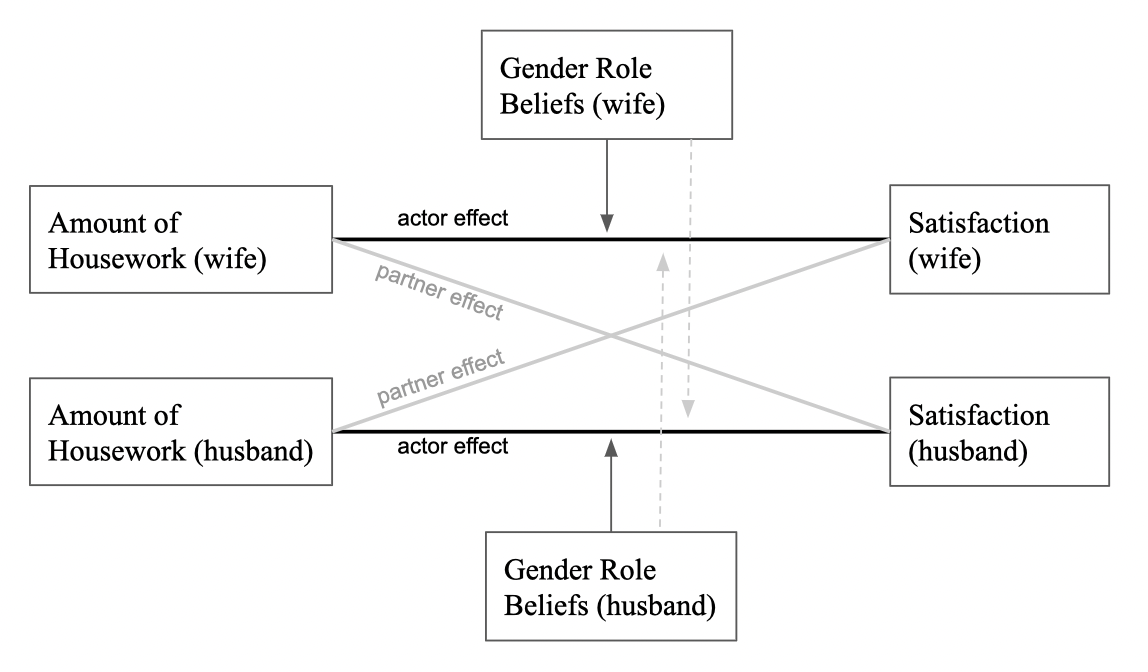
\includegraphics[width=3.83in]{APIM} \caption{Schematic representation of actor and partner effects in the APIM moderated by gender role beliefs.}\label{fig:unnamed-chunk-47}
\end{figure}

\hypertarget{main-results}{%
\subsection{Main Results}\label{main-results}}

\hypertarget{gender-role-beliefs-1}{%
\paragraph{Gender Role Beliefs}\label{gender-role-beliefs-1}}

All relevant results of the moderation analysis in the APIM are shown in figure 2. It was shown that for husbands and wives, a higher amount of housework was significantly related to a lower satisfaction. For wives we found \(\beta\) =-0.02, \emph{p} = 0.02, and SE =0.01. For husbands we found \(\beta\) =-0.03, \emph{p} = 0.01 and SE = 0.01.
For the female partners, their own gender role beliefs significantly moderated the relationship between their housework distribution and their satisfaction with the housework distribution. The moderation effect was 0.07 (\emph{p} = \textless0.01, SE = 0.02). When the wives had higher gender role beliefs, which means more conservative, their satisfaction with the housework distribution tended to be higher, while keeping their own housework distribution constant at the mean. The husband's gender role beliefs significantly moderated the relationship between the wife's housework distribution and the wife's satisfaction with the housework distribution. The moderation effect was -0.06 (\emph{p} = 0.01, SE = 0.02). When the husbands had more conservative gender role beliefs, the wife's satisfaction decreased by -0.06 while keeping the wives housework distribution constant at the mean. Moreover, a marginally significant moderation effect was found for the relationship between the husbands amount of housework and the wife's satisfaction which was moderated by the wife's gender role beliefs (\(\beta\) = 0.03, \emph{p} =0.10, SE = 0.02). When wives had more conservative gender role beliefs, their satisfaction tended to be higher, while their husbands housework distribution was held constant at the mean.




\begin{figure}
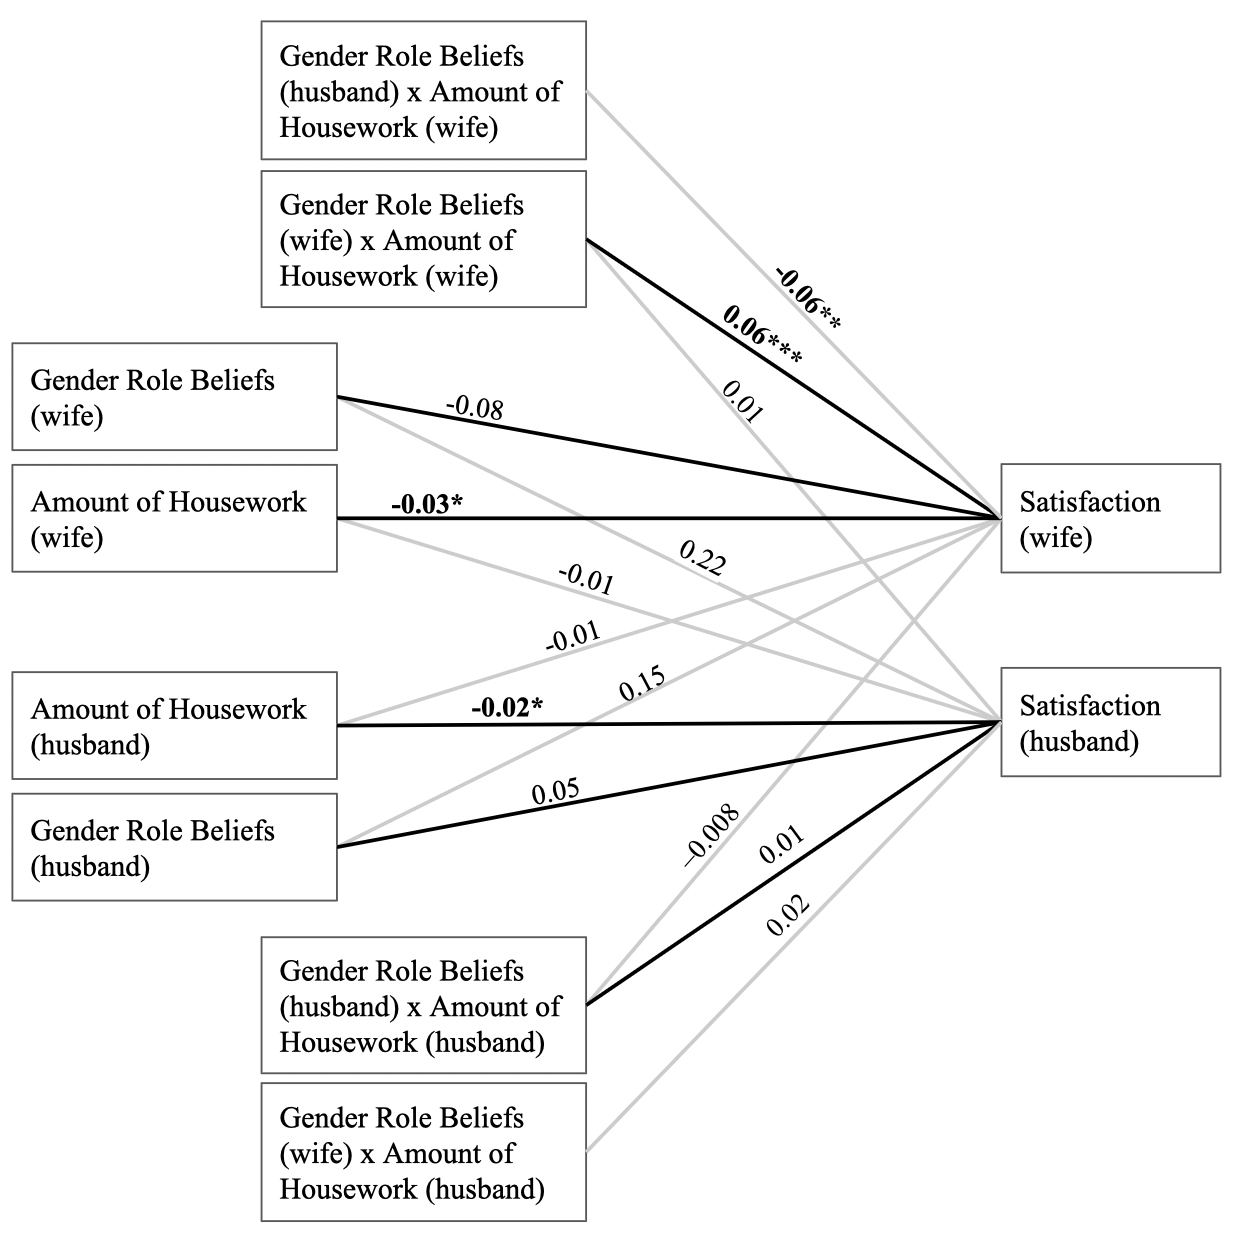
\includegraphics[width=4.11in]{moderation} \caption{Moderation effects in the APIM. Values shown in the figure are \(\beta\) coefficients.
* \emph{p} \textless{} .05, ** \emph{p} \textless{} .01, *** \emph{p} \textless{} .001.}\label{fig:unnamed-chunk-53}
\end{figure}



\begin{figure}
\centering
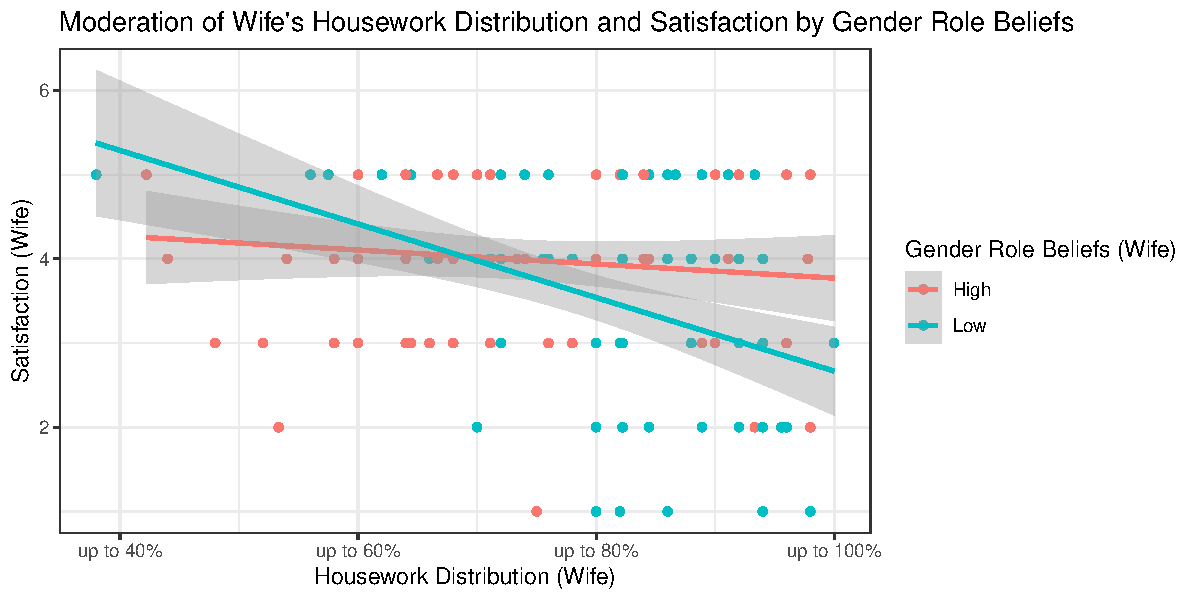
\includegraphics{Final_Paper_files/figure-latex/unnamed-chunk-56-1.pdf}
\caption{\label{fig:unnamed-chunk-56}Moderation of wife's housework distribution and satisfaction by gender role beliefs. Housework distribution in \%, Satisfaction and gender role beliefs were measured with a 5 point Likert scale (1 = liberal, 5 = conservative).}
\end{figure}



\begin{figure}
\centering
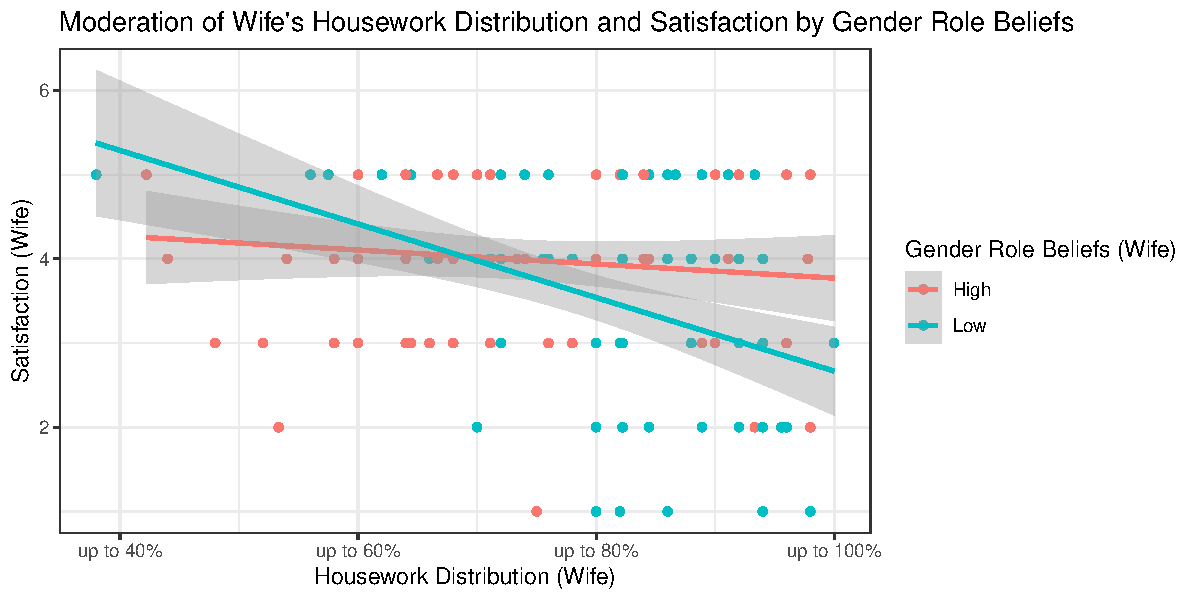
\includegraphics{Final_Paper_files/figure-latex/unnamed-chunk-57-1.pdf}
\caption{\label{fig:unnamed-chunk-57}Moderation of wife's housework distribution and her satisfaction by their husbands gender role beliefs. Housework distribution in \%, Satisfaction and gender role beliefs were measured with a 5 point Likert scale (1 = liberal, 5 = conservative).}
\end{figure}

Wives who have low gender role beliefs, which means they are more liberal, reported a lower satisfaction with an increasing amount of housework they had to do. Women with more conservative gender role beliefs (high value) did not show a significant decrease in satisfaction with an increasing amount of housework (figure 3).

As the the amount of housework increases for wives whose husbands have low gender role beliefs, their satisfaction remains constant. When housework increases for wives whose husbands have high gender role beliefs, their satisfaction decreases (figure 4).
Since we used distinguishable dyads, gender was a built in moderator. To see if the moderation effects differed significantly by gender, we looked at the three way interactions between gender, housework distribution, and gender role beliefs. We found two significant gender differences in the moderation effects. The interaction between the actor's housework and their own gender role beliefs was significantly different for husbands and wives with an estimate of 0.06 (\emph{p} = 0.03, SE = 0.03). The moderation effect of ones own gender role beliefs was 0.06 units higher for women than men, meaning the moderation effect of gender role beliefs had a significantly larger positive effect on satisfaction for wives than for husbands.
In addition, the interaction between the actor's amount of housework and their partners gender role beliefs was significantly different for husbands and wives with an estimate of -0.08(\emph{p} = 0.01, SE = 0.03).The moderation effect of the partners gender role beliefs was -0.08 units lower for women than men which means that the moderation effect of the husbands gender role beliefs had a significantly larger negative effect on satisfaction compared to how the wifes gender role beliefs effected the relationship between housework distribution and satisfaction for her husband.

\hypertarget{religion}{%
\paragraph{Religion}\label{religion}}

No significant relationships between any of the variables have been found in the APIM model including the moderator religion (\emph{p} \textgreater{} 0.19). Religion did therefore not moderate the relationship between housework distribution and satisfaction for wives and husbands.

\hypertarget{exploratory-results}{%
\subsection{Exploratory Results}\label{exploratory-results}}

In order to being able to find possible explanations for the association between gender role beliefs and satisfaction that we found in our analysis, we conducted a simple mediation analysis, investigating whether the wife's gatekeeping mediated the relationship between her gender role beliefs and her satisfaction, and therefore could explain the patterns found in the prior analysis. Are women with higher gender role beliefs more likely to gatekeep housework tasks which would in turn lead to a higher satisfaction?
Linear models will be calculated for all paths to see whether all paths are significant first, before we will calculate the mediation effect in a second step.




\begin{figure}
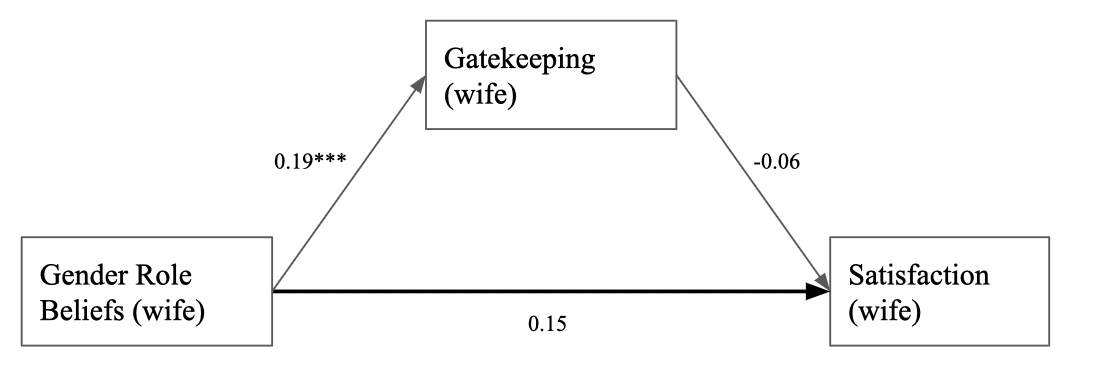
\includegraphics[width=3.69in]{mediation} \caption{Proposed mediation model with wife's gatekeeping as the mediator of the wife's gender role beliefs and satisfaction. Values shown in the figure are \(\beta\) coefficients.
* \emph{p} \textless{} .05, ** \emph{p} \textless{} .01, *** \emph{p} \textless{} .001.}\label{fig:unnamed-chunk-63}
\end{figure}

As seen in figure 5, no significant relationship between gender role beliefs and satisfaction has been found, despite the moderating effect of gender role beliefs that has been found before. Because only the relationship between gender role beliefs and gatekeeping has been significant, a full mediation analysis was no longer appropriate to conduct.
Instead, we conducted post-hoc t tests to get a better sense of the relationship between gender role beliefs and gatekeeping. INCLUDE T TESTS HERE.

\#Discussion

\newpage

\hypertarget{references}{%
\section{References}\label{references}}

\hypertarget{refs}{}
\begin{CSLReferences}{1}{0}
\leavevmode\vadjust pre{\hypertarget{ref-hawkins_1999}{}}%
Allen, S. M., \& Hawkins, A. J. (1999). \emph{Maternal gatekeeping: Mothers' beliefs and behaviors that inhibit greater father involvement in family work}. Retrieved from \url{https://doi.org/10.2307/353894}

\leavevmode\vadjust pre{\hypertarget{ref-R-papaja}{}}%
Aust, F., \& Barth, M. (2020). \emph{{papaja}: {Create} {APA} manuscripts with {R Markdown}}. Retrieved from \url{https://github.com/crsh/papaja}

\leavevmode\vadjust pre{\hypertarget{ref-baxter_western_1998}{}}%
Baxter, J., \& Western, M. (1998). \emph{Satisfaction with housework: Examining the paradox.} Retrieved from \url{https://doi.org/10.1177/0038038598032001007}

\leavevmode\vadjust pre{\hypertarget{ref-benin_agostinelli_1988}{}}%
Benin, M. H., \& Agostinelli, J. (1988). \emph{Husbands' and wives satisfaction with the division of labor}. Retrieved from \url{https://doi.org/10.2307/352002}

\leavevmode\vadjust pre{\hypertarget{ref-bird_99}{}}%
Bird, C. E. (1999). \emph{Gender, household labor, and psychological distress: The impact of the amount and division of housework}. Retrieved from \url{https://doi.org/10.2307/2676377}

\leavevmode\vadjust pre{\hypertarget{ref-blair_lichter_1999}{}}%
Blair, S., \& Lichter, D. (1999). \emph{Measuring the division of household labor: Gender segregation of housework among american couples}. Retrieved from \url{https://doi.org/10.1177/019251391012001007}

\leavevmode\vadjust pre{\hypertarget{ref-buunk_2000}{}}%
Buunk, B. P., Kluwer, E. S., Schuurman, M. K., \& Siero, F. W. (2000). The division of labor among egalitarian and traditional women: Differences in discontent, social comparison, and false consensus. In \emph{Journal of Applied Social Psychology} (No. 4; Vol. 30, pp. 759--779). Wiley Online Library.

\leavevmode\vadjust pre{\hypertarget{ref-charbonneau_2019}{}}%
Charbonneau, A., Lachance-Grzela1, M., \& Bouchard1, G. (2019). \emph{Housework allocation, negotiation strategies, and relationship satisfaction in cohabiting emerging adult heterosexual couples}. Retrieved from \url{https://doi.org/10.1007/s11199-018-0998-1}

\leavevmode\vadjust pre{\hypertarget{ref-demaris_2010}{}}%
DeMaris, A. (2010). \emph{The 20-year trajectory of marital quality in enduring marriages: Does equity matter?} Retrieved from \url{https://dx.doi.org/10.1177\%2F0265407510363428}

\leavevmode\vadjust pre{\hypertarget{ref-demaris_2013}{}}%
DeMaris, A., Mahoney, A., \& Pargament, K. (2013). \emph{Fathers' contributions to housework and childcare and parental aggravation amongst first-time parents}. Retrieved from \url{https://doi.org/10.3149/fth.1102.179}

\leavevmode\vadjust pre{\hypertarget{ref-ellison_bartkowski_2002}{}}%
Ellison, C., \& Bartkowski, J. (2002). \emph{Conservative protestantism and the division of household labor among married couples}. Retrieved from \url{https://doi.org/10.1177/019251302237299}

\leavevmode\vadjust pre{\hypertarget{ref-evertson_2014}{}}%
Evertsson, M. (2014). Gender ideology and the sharing of housework and child care in sweden. In \emph{Journal of Family Issues} (No. 7; Vol. 35, pp. 927--949). Sage Publications Sage CA: Los Angeles, CA.

\leavevmode\vadjust pre{\hypertarget{ref-forste_fox_2008}{}}%
Forste, R., \& Fox, K. (2008). \emph{Household labor, gender roles, and family satisfaction: A cross-national comparison}. Retrieved from \url{https://www.jstor.org/stable/23267837}

\leavevmode\vadjust pre{\hypertarget{ref-forste_fox_2012}{}}%
Forste, \& Fox. (2012). \emph{Household labor, gender roles, and family satisfaction: A cross-national comparison}. Retrieved from \url{https://www.jstor.org/stable/23267837}

\leavevmode\vadjust pre{\hypertarget{ref-glass_fujimoto_94}{}}%
Glass, J., \& Fujimoto, T. (1994). \emph{Housework, paid work, and depression among husbands and wives}. Retrieved from \url{https://www.jstor.org/stable/2137364}

\leavevmode\vadjust pre{\hypertarget{ref-goldschneider_2014}{}}%
Goldscheider, F. G. C., \& Rico-Gonzalez3, A. (2014). \emph{Gender equality in sweden: Are the religious more patriarchal?} Retrieved from \url{https://doi.org/10.1177/0192513X14522236}

\leavevmode\vadjust pre{\hypertarget{ref-greenstein_1996}{}}%
Greenstein, T. N. (1996). \emph{Husbands' participation in domestic labor: Interactive effects of wives' and husbands' gender ideologies}. Retrieved from \url{https://doi.org/10.2307/353719}

\leavevmode\vadjust pre{\hypertarget{ref-gull_geist_2020}{}}%
Gull, B., \& Geist, C. (2020). \emph{Godly husbands and housework: A global examination of the association between religion and men's housework participation.}

\leavevmode\vadjust pre{\hypertarget{ref-hunt_jung_2009}{}}%
Hunt, M., \& Jung, P. (2009). \emph{'Good sex' and religion: A feminist overview}. Retrieved from \url{https://www.jstor.org/stable/20620412}

\leavevmode\vadjust pre{\hypertarget{ref-kenny2020dyadic}{}}%
Kenny, D. A., Kashy, D. A., \& Cook, W. L. (2020). \emph{Dyadic data analysis}. Guilford Publications.

\leavevmode\vadjust pre{\hypertarget{ref-catholic_league_pope_2020}{}}%
League, C. (2020). Pope brands transgender theory as evil. Retrieved from \url{https://www.catholicleague.org/pope-brands-transgender-theory-as-evil-2/}

\leavevmode\vadjust pre{\hypertarget{ref-leopold_2019}{}}%
Leopold. (2019). \emph{Diverging trends in satisfaction with housework: Declines in women, increases in men}. Retrieved from \url{http://dx.doi.org/10.1111/jomf.12520}

\leavevmode\vadjust pre{\hypertarget{ref-mikula_1997}{}}%
Mikula, G., Freudenthaler, H. H., Brennacher-Kroll, S., \& Brunschko, B. (1997). Division of labor in student households: Gender inequality, perceived justice, and satisfaction. In \emph{Basic and Applied Social Psychology} (No. 3; Vol. 19, pp. 275--289). Taylor \& Francis.

\leavevmode\vadjust pre{\hypertarget{ref-musek_2017}{}}%
Musek, J. (2017). \emph{Values related to the religious adherence}. Retrieved from \url{https://doi.org/10.31820/pt.26.2.10}

\leavevmode\vadjust pre{\hypertarget{ref-nelson_1977}{}}%
Nelson, E. N. (1977). \emph{Women's work -- housework alientation}. Retrieved from \url{https://www.jstor.org/stable/23261802}

\leavevmode\vadjust pre{\hypertarget{ref-okulicz_valente_2018}{}}%
Okulicz-Kozaryn, A., \& Rocha Valente, R. da. (2018). \emph{Life satisfaction of career women and housewives}. Retrieved from \url{https://doi.org/10.1007/s11482-017-9547-2}

\leavevmode\vadjust pre{\hypertarget{ref-R-base}{}}%
R Core Team. (2020). \emph{R: A language and environment for statistical computing}. Vienna, Austria: R Foundation for Statistical Computing. Retrieved from \url{https://www.R-project.org/}

\leavevmode\vadjust pre{\hypertarget{ref-ruppanner_2012}{}}%
Ruppanner, L. (2012). \emph{Housework conflict and divorce: A multi-level analysis}. Retrieved from \url{https://www.jstor.org/stable/43497126}

\leavevmode\vadjust pre{\hypertarget{ref-spitze_loscocco_2000}{}}%
Spitze, G., \& Loscocco, K. A. (2000). \emph{The labor of sisyphus? Women's and men's reactions to housework}. Retrieved from \url{https://www.jstor.org/stable/42864042}

\end{CSLReferences}


\clearpage
\renewcommand{\listfigurename}{Figure captions}

\clearpage
\renewcommand{\listtablename}{Table captions}


\end{document}
